\documentclass[conference]{IEEEtran}
\IEEEoverridecommandlockouts
\usepackage{cite}
\usepackage{amsmath,amssymb,amsfonts}
\usepackage{algorithmic}
\usepackage{algorithm}
\usepackage{graphicx}
\graphicspath{{./}{figures/}{./figures/}}
\usepackage{textcomp}
\usepackage{xcolor}
\usepackage{tikz}
\usetikzlibrary{shapes.geometric,arrows.meta,positioning,fit,backgrounds,calc,shadows}
\usepackage{booktabs}
\usepackage{array}
\usepackage{url}
\def\BibTeX{{\rm B\kern-.05em{\sc i\kern-.025em b}\kern-.08em
    T\kern-.1667em\lower.7ex\hbox{E}\kern-.125emX}}

\begin{document}

\title{XAI-MedVision: A Multi-Specialty Clinical Decision Support System with Explainable AI\\
}

\author{
\begin{tabular}[t]{c@{\hskip 0.03\textwidth}c@{\hskip 0.03\textwidth}c}
\begin{minipage}[t]{0.30\textwidth}\centering
Pilli Sai Medhas\\
\textit{Dept. of Computer Science and Engineering}\\
\textit{(Artificial Intelligence and Machine Learning)}\\
\textit{Vel Tech Rangarajan Dr. Sagunthala}\\
\textit{R\&D Institute of Science and Technology}\\
Chennai, Tamil Nadu, India\\
vtu24914@veltech.edu.in
\end{minipage}
&
\begin{minipage}[t]{0.30\textwidth}\centering
Jammula Rithik Reddy\\
\textit{Dept. of Computer Science and Engineering}\\
\textit{(Artificial Intelligence and Machine Learning)}\\
\textit{Vel Tech Rangarajan Dr. Sagunthala}\\
\textit{R\&D Institute of Science and Technology}\\
Chennai, Tamil Nadu, India\\
vtu25092@veltech.edu.in
\end{minipage}
&
\begin{minipage}[t]{0.30\textwidth}\centering
P. S. Apirajitha\\
\textit{Assistant Professor Senior Grade}\\
\textit{Dept. of Computer Science and Engineering}\\
\textit{Vel Tech Rangarajan Dr. Sagunthala}\\
\textit{R\&D Institute of Science and Technology}\\
Chennai, Tamil Nadu, India\\
apirajitha.s@gmail.com
\end{minipage}
\end{tabular}
}

\maketitle

% ============================================================
% ABSTRACT
% ============================================================
\begin{abstract}
Modern clinical diagnostic workflows require rapid, accurate multi-modal interpretation of medical imaging and patient health records. However, deep neural networks often function as opaque black boxes, limiting clinical trust and hindering deployment in high-stakes healthcare environments. In this paper, we present \textbf{XAI-MedVision}, an end-to-end, multi-specialty Clinical Decision Support System (CDSS) that seamlessly integrates vision-based diagnostic engines with visual explainability and automated Natural Language Processing (NLP) report generation. Our platform features a smart modality router that dynamically dispatches patient scans to four specialized vision models: EfficientNet-B0 for Brain Tumor MRI classification (98.40\% accuracy), ResNet-50 for Musculoskeletal Bone Fracture detection (97.60\% accuracy), DenseNet-121 for Pulmonary Pneumonia screening on Chest X-Rays (95.80\% accuracy), and MobileNetV2 for Complete Blood Count (CBC) hematology profiling (96.20\% accuracy). To provide visual interpretability, the pipeline incorporates Gradient-weighted Class Activation Mapping (Grad-CAM), generating precise pixel-level saliency heatmaps that highlight anatomical lesions and abnormal cellular structures. Furthermore, an adapted FLAN-T5 Seq2Seq model fine-tuned with Low-Rank Adaptation (LoRA) automatically synthesizes raw diagnostic predictions and clinical notes into structured discharge summaries, achieving high textual fidelity (ROUGE-1: 44.82\%, ROUGE-2: 24.15\%, ROUGE-L: 41.56\%). Profiled on standard CPU hardware, the complete vision inference latency remains under 135\,ms per image with total model parameter storage requiring less than 150\,MB, establishing XAI-MedVision as an efficient, transparent, and deployment-ready computational aid for modern medical triage.
\end{abstract}

\begin{IEEEkeywords}
Clinical Decision Support System, Explainable AI, Grad-CAM, Deep Learning, Medical Imaging, Transfer Learning, FLAN-T5, LoRA Summarization, Multi-Specialty Healthcare
\end{IEEEkeywords}

% ============================================================
% I. INTRODUCTION
% ============================================================
\section{Introduction}
Medical imaging and clinical text analysis form the bedrock of contemporary disease diagnosis and patient management. Radiologists, oncologists, and clinicians evaluate thousands of high-resolution images daily---ranging from magnetic resonance imaging (MRI) and digital radiography to microscopic hematology slides---alongside dense electronic health records (EHRs). The exponential increase in patient volume, coupled with clinician burnout and diagnostic fatigue, creates an urgent demand for automated, highly reliable Clinical Decision Support Systems (CDSS).

\begin{figure}[htbp]
\centering
\IfFileExists{fig1_ui_interface.png}{%
    \includegraphics[width=\columnwidth]{fig1_ui_interface.png}%
}{%
    \IfFileExists{figures/fig1_ui_interface.png}{%
        \includegraphics[width=\columnwidth]{figures/fig1_ui_interface.png}%
    }{%
        \fbox{\parbox{0.92\columnwidth}{\centering\vspace{14pt}\textbf{[ Figure 1: XAI-MedVision Client Interface ]}\\\vspace{4pt}\texttt{fig1\_ui\_interface.png}\\\vspace{14pt}}}%
    }%
}
\caption{XAI-MedVision web dashboard demonstrating multi-modal patient scan ingestion, real-time Grad-CAM saliency map visualization, and automated T5 clinical discharge report generation.}
\label{fig:system_ui}
\end{figure}

Despite remarkable breakthroughs in deep convolutional neural networks (CNNs) for medical image classification, conventional computer-assisted diagnostic tools suffer from two fundamental bottlenecks:
\begin{enumerate}
    \item \textbf{The Interpretability Gap:} Standard deep learning architectures operate as opaque mathematical models, offering output probabilities without spatial or contextual justification. Medical professionals cannot audit the underlying decision criteria, leading to skepticism and regulatory hurdles.
    \item \textbf{Isolated Task Specialization:} Most existing CDSS tools focus exclusively on single modalities (e.g., chest radiography only) or provide raw classification labels without synthesizing actionable, structured clinical reports.
\end{enumerate}

To bridge these critical research gaps, we present \textbf{XAI-MedVision}, a full-stack, multi-specialty clinical decision support platform. As illustrated in Fig.~\ref{fig:system_ui}, XAI-MedVision combines specialized vision backbones (EfficientNet-B0, ResNet-50, DenseNet-121, MobileNetV2) with Gradient-weighted Class Activation Mapping (Grad-CAM) and parameter-efficient NLP report generation using FLAN-T5 fine-tuned via Low-Rank Adaptation (LoRA). 

The primary contributions of this work are summarized as follows:
\begin{itemize}
    \item \textbf{Multi-Specialty Routing Architecture:} We engineer a unified intake engine that routes patient inputs across four diverse clinical specialties: neuro-oncology (Brain MRI), orthopedics (Bone Fracture X-Ray), pulmonology (Chest X-Ray), and hematology (CBC Blood Cells).
    \item \textbf{Transparent Visual Explanations:} We embed Grad-CAM saliency heatmaps into every vision diagnostic module, providing radiologists with immediate pixel-level visual validation of identified pathologies.
    \item \textbf{Automated Clinical Report Synthesis:} We implement a FLAN-T5 LoRA language model fine-tuned on MIMIC-III clinical discharge records to translate multi-modal diagnostic predictions into structured 3-part medical summaries.
    \item \textbf{Edge-Ready Latency & Footprint:} We optimize all model pipelines for CPU deployment, achieving an average per-image inference speed of 45.17--132.75\,ms while maintaining a total checkpoint footprint of under 150\,MB.
\end{itemize}

% ============================================================
% II. LITERATURE SURVEY
% ============================================================
\section{Literature Survey}
In this section, we analyze fifteen prominent peer-reviewed studies published between 2017 and 2025 across medical computer vision, explainable AI, and clinical natural language processing, highlighting how XAI-MedVision addresses current methodological limitations.

\subsection{Deep Learning in Medical Vision}
Deep convolutional networks have achieved diagnostic parity with human experts in specialized domains. Rajpurkar et al.~\cite{b1} developed CheXNet using DenseNet-121 to detect pneumonia from chest radiographs, exceeding average radiologist performance. Tan and Le~\cite{b6} introduced EfficientNet, demonstrating superior scaling for image classification, which Nickparvar~\cite{b9} applied to brain MRI tumor classification. He et al.~\cite{b7} established ResNet architectures for feature extraction, while Sandler et al.~\cite{b8} engineered MobileNetV2 for lightweight, resource-constrained vision tasks. Esteva et al.~\cite{b12} and Kermany et al.~\cite{b13} demonstrated dermatological and retinal diagnostic pipelines using transfer learning. Litjens et al.~\cite{b14} provided a comprehensive survey of deep learning in medical image analysis, noting the predominance of single-task models.

\subsection{Explainable AI (XAI) in Healthcare}
Visual interpretability is paramount in clinical environments. Selvaraju et al.~\cite{b2} introduced Grad-CAM, utilizing class-specific gradient information flowing into the final convolutional layer to produce localization maps. Lundberg and Lee~\cite{b3} developed SHAP (SHapley Additive exPlanations) to measure feature importance. Tjoa and Guan~\cite{b15} surveyed medical XAI methods, emphasizing that explainability builds clinical trust and helps detect dataset bias. However, most existing XAI systems remain academic prototypes disconnected from user-facing report generation tools.

\subsection{Clinical NLP & Automated Report Generation}
Processing unstructured electronic health records (EHR) has advanced significantly with transformer architectures. Raffel et al.~\cite{b4} presented the Text-to-Text Transfer Transformer (T5), establishing strong benchmarks for text summarization. To fine-tune large transformers efficiently on clinical datasets such as MIMIC-III (Johnson et al.~\cite{b11}), Hu et al.~\cite{b5} proposed Low-Rank Adaptation (LoRA), which freezes pretrained model weights and injects trainable rank decomposition matrices. Mooney~\cite{b10} curated open medical datasets for pneumonia and blood cell classification, facilitating benchmarking.

\subsection{Comparative Literature Analysis}
Table~\ref{tab:litsurvey} provides a comparative analysis of XAI-MedVision against landmark baseline literature across diagnostic modalities, explainability support, and report generation capabilities.

\begin{table}[htbp]
\caption{Comparative Summary: Existing Literature vs. Proposed XAI-MedVision System}
\label{tab:litsurvey}
\centering
\setlength{\tabcolsep}{3pt}
\footnotesize
\begin{tabular}{|>{\raggedright\arraybackslash}p{1.8cm}|>{\raggedright\arraybackslash}p{2.2cm}|>{\centering\arraybackslash}p{1.2cm}|>{\centering\arraybackslash}p{1.0cm}|>{\centering\arraybackslash}p{0.8cm}|}
\hline
\textbf{Work} & \textbf{Modality Scope} & \textbf{Primary Model} & \textbf{XAI Method} & \textbf{NLP Report} \\
\hline
Rajpurkar et al.~\cite{b1} & Chest X-Ray & DenseNet-121 & CAM & No \\
Selvaraju et al.~\cite{b2} & General Vision & VGG/ResNet & Grad-CAM & No \\
Lundberg et al.~\cite{b3} & Tabular / Vision & SHAP & Feature Shapley & No \\
Raffel et al.~\cite{b4} & Text Summarization & T5 Seq2Seq & None & Yes \\
Nickparvar~\cite{b9} & Brain MRI & EfficientNet & None & No \\
Kermany et al.~\cite{b13} & OCT / Chest X-Ray & InceptionV3 & Occlusion & No \\
Litjens et al.~\cite{b14} & Medical Vision Survey & Multi-CNN & None & No \\
\hline
\textbf{XAI-MedVision (Ours)} & \textbf{Brain MRI, Bone X-Ray, Chest X-Ray, Blood CBC} & \textbf{EfficientNet, ResNet, DenseNet, MobileNet, FLAN-T5} & \textbf{Grad-CAM \& SHAP} & \textbf{Yes (LoRA T5)} \\
\hline
\end{tabular}
\end{table}

% ============================================================
% III. PROBLEM STATEMENT
% ============================================================
\section{Problem Statement}
Deploying artificial intelligence tools into routine hospital workflows faces four critical challenges:
\begin{enumerate}
    \item \textbf{Lack of Spatial Accountability:} Standard deep networks output scalar confidence scores (e.g., ``Pneumonia 98.2\%'') without revealing which image regions generated the score. False positives caused by background artifacts remain undetected.
    \item \textbf{Fragmentation across Clinical Departments:} Current AI applications require separate software instances for neurology, orthopedics, pulmonology, and pathology, creating operational overhead for medical IT staff.
    \item \textbf{Unstructured Output & Manual Documentation:} Clinicians must manually copy AI predictions into EHR systems, increasing documentation time and risking transcript errors.
    \item \textbf{High Compute & Latency Overhead:} Large vision-language models frequently require expensive GPU hardware, rendering them impractical for low-resource rural health centers and mobile diagnostic units.
\end{enumerate}

XAI-MedVision addresses these limitations by pairing modular multi-specialty neural networks with automated Grad-CAM saliency heatmaps and an edge-optimized FLAN-T5 LoRA clinical summarizer.

% ============================================================
% IV. SYSTEM OVERVIEW
% ============================================================
\section{Implemented System Overview}
The XAI-MedVision framework operates as a fully integrated web platform engineered using FastAPI, PyTorch, HuggingFace Transformers, and modern client-side technologies.

\subsection{Input Ingestion & Modality Preprocessing}
When a medical scan or clinical note is uploaded through the dashboard, the system inspects image metadata and dimensional properties. Images are resized to $224 \times 224 \times 3$ resolution, converted to standard RGB tensor representations, and normalized using ImageNet channel statistics ($\mu = [0.485, 0.456, 0.406]$, $\sigma = [0.229, 0.224, 0.225]$).

\subsection{Multi-Specialty Vision Diagnostic Modules}
\begin{itemize}
    \item \textbf{Brain MRI Module (EfficientNet-B0):} Evaluates cranial MRI slices to classify scans into four categories: Glioma, Meningioma, Pituitary Tumor, or No Tumor.
    \item \textbf{Bone Fracture Module (ResNet-50):} Analyzes musculoskeletal X-rays across multi-region appendicular fractures (Fractured vs. Non-Fractured).
    \item \textbf{Chest X-Ray Module (DenseNet-121):} Evaluates pulmonary X-rays for inflammatory lung consolidation (Normal vs. Pneumonia).
    \item \textbf{Hematology Blood Cell Module (MobileNetV2):} Performs Complete Blood Count cell differential profiling across four distinct white blood cell categories: Eosinophil, Lymphocyte, Monocyte, and Neutrophil.
\end{itemize}

\subsection{Visual Explainability Engine}
For every visual diagnosis, the system invokes PyTorch Grad-CAM to compute the gradient of the predicted class score with respect to feature maps in the final convolutional layer. The resulting activation map is upsampled to original image dimensions, normalized, and rendered as a high-contrast Jet colormap overlay.

\subsection{Automated NLP Summarization Engine}
To generate clinical summaries, raw patient notes and diagnostic outputs are ingested by a fine-tuned FLAN-T5 model equipped with LoRA adapters. The model outputs a structured three-section clinical record comprising:
\begin{enumerate}
    \item \textbf{[1] Key Diagnostic Findings}
    \item \textbf{[2] In-Hospital Treatment Summary}
    \item \textbf{[3] Post-Discharge Follow-Up Plan}
\end{enumerate}

% ============================================================
% V. DATASET COMPOSITION AND TRAINING METHODOLOGY
% ============================================================
\section{Dataset Composition and Training Methodology}

\subsection{Dataset Curation}
Our models were trained, validated, and evaluated on five benchmark medical datasets comprising a total of \textbf{28,961 curated samples}. Table~\ref{tab:dataset} details the class distributions and split allocations.

\begin{table}[htbp]
\caption{Dataset Partitioning and Specialty Class Distributions}
\label{tab:dataset}
\centering
\setlength{\tabcolsep}{3pt}
\footnotesize
\begin{tabular}{|>{\raggedright\arraybackslash}p{1.8cm}|>{\centering\arraybackslash}p{1.1cm}|>{\centering\arraybackslash}p{0.9cm}|>{\raggedright\arraybackslash}p{3.2cm}|}
\hline
\textbf{Specialty Split} & \textbf{Samples} & \textbf{Classes} & \textbf{Target Pathology / Categories} \\
\hline
Brain Tumor MRI & 7,023 & 4 & Glioma, Meningioma, Pituitary, No Tumor \\
\hline
Bone Fracture & 10,582 & 2 & Fractured, Not Fractured \\
\hline
Chest X-Ray & 5,856 & 2 & Normal, Pneumonia \\
\hline
Blood Cell CBC & 12,500 & 4 & Eosinophil, Lymphocyte, Monocyte, Neutrophil \\
\hline
MIMIC-III Summaries & 300 & Seq2Seq & Clinical Discharge Note Summaries \\
\hline
\textbf{Total Corpus} & \textbf{36,261} & {--} & {--} \\
\hline
\end{tabular}
\end{table}

\subsection{Data Augmentation & Class Imbalance Mitigation}
To prevent overfitting on medical imaging splits, we applied domain-specific stochastic transformations during training:
\begin{itemize}
    \item Random horizontal/vertical flipping ($p=0.5$).
    \item Affine rotations ($\pm 10^\circ$ to $\pm 20^\circ$) and scaling variations ($0.96\times$--$1.04\times$).
    \item Color jittering (brightness $\pm 0.15$, contrast $\pm 0.15$).
\end{itemize}
To address dataset class imbalance, we applied class-weighted cross-entropy loss formulation:
\begin{equation}
w_j = \frac{N}{C \cdot n_j}
\end{equation}
where $N$ is total training instances, $C$ is class count, and $n_j$ is the frequency of sample class $j$.

\subsection{Optimization & Scheduling}
All models were optimized using AdamW with weight decay $\lambda = 10^{-4}$. Learning rates were dynamically adjusted using Cosine Annealing with Warm Restarts over 10 training epochs ($\eta_{max} = 2 \times 10^{-4}$, $\eta_{min} = 10^{-6}$). Label smoothing ($\epsilon = 0.05$--$0.10$) was incorporated into loss functions to prevent overconfidence in logit predictions.

% ============================================================
% VI. SYSTEM ARCHITECTURE AND WORKFLOW
% ============================================================
\section{System Architecture \& Workflow}
Fig.~\ref{fig:architecture} presents the end-to-end multi-tier pipeline of XAI-MedVision, mapping data flow from client ingestion through modality routing, neural feature extraction, Grad-CAM heatmap generation, and T5 report synthesis.

\begin{figure*}[!t]
\centering
\IfFileExists{fig2_architecture.png}{%
    \includegraphics[width=0.98\textwidth]{fig2_architecture.png}%
}{%
    \IfFileExists{figures/fig2_architecture.png}{%
        \includegraphics[width=0.98\textwidth]{figures/fig2_architecture.png}%
    }{%
        \begin{tikzpicture}[
            node distance=1.2cm and 1.0cm,
            box/.style={draw=blue!80!black, fill=blue!10, rounded corners=6pt, thick, align=center, minimum height=1.1cm, minimum width=2.4cm, font=\sffamily\small},
            router/.style={draw=orange!80!black, fill=orange!15, rounded corners=6pt, thick, align=center, minimum height=1.1cm, minimum width=2.4cm, font=\sffamily\small},
            vision/.style={draw=green!80!black, fill=green!15, rounded corners=6pt, thick, align=center, minimum height=1.1cm, minimum width=2.5cm, font=\sffamily\small},
            xai/.style={draw=purple!80!black, fill=purple!15, rounded corners=6pt, thick, align=center, minimum height=1.1cm, minimum width=2.4cm, font=\sffamily\small},
            nlp/.style={draw=violet!80!black, fill=violet!15, rounded corners=6pt, thick, align=center, minimum height=1.1cm, minimum width=2.4cm, font=\sffamily\small},
            dash/.style={draw=red!80!black, fill=red!15, rounded corners=6pt, thick, align=center, minimum height=1.1cm, minimum width=2.4cm, font=\sffamily\small},
            arrow/.style={->, >=Stealth, thick, color=gray!80!black}
        ]
            \node (ingest) [box] {\textbf{Intake Gateway}\\Patient Scan / EHR};
            \node (route) [router, right=of ingest] {\textbf{Smart Modality Router}\\Modality Selection};
            \node (vis) [vision, right=of route] {\textbf{Specialist Vision Engines}\\EfficientNet / ResNet /\\DenseNet / MobileNet};
            \node (cam) [xai, above right=0.3cm and 0.8cm of vis] {\textbf{Grad-CAM Explainer}\\Saliency Heatmap Overlay};
            \node (t5) [nlp, below right=0.3cm and 0.8cm of vis] {\textbf{FLAN-T5 Generator}\\LoRA Seq2Seq Summary};
            \node (ui) [dash, right=3.6cm of vis] {\textbf{Physician Review}\\Interactive Dashboard};

            \draw [arrow] (ingest) -- (route);
            \draw [arrow] (route) -- (vis);
            \draw [arrow] (vis) |- (cam);
            \draw [arrow] (vis) |- (t5);
            \draw [arrow] (cam) -| (ui);
            \draw [arrow] (t5) -| (ui);
        \end{tikzpicture}
    }%
}
\caption{System Architecture of XAI-MedVision: Modular multi-tier pipeline including client intake gateway, smart modality routing, specialist neural vision engines, Grad-CAM explainability, FLAN-T5 LoRA clinical summarization, and physician review dashboard.}
\label{fig:architecture}
\end{figure*}

% ============================================================
% VII. ALGORITHMS
% ============================================================
\section{Algorithms}

\subsection{Transfer Learning and Optimization Pipeline}
Algorithm~\ref{alg:train} details the formal training procedure with label smoothing, class weighting, and Cosine Annealing learning rate scheduling.

\begin{algorithm}[htbp]
\caption{Transfer Learning \& Optimization Pipeline}
\label{alg:train}
\begin{algorithmic}[1]
\REQUIRE Training set $\mathcal{D}_{tr}$, Validation set $\mathcal{D}_{val}$, Pretrained model backbone $\mathcal{M}_0$, Epochs $E$, Initial LR $\eta_0$, Label smoothing $\epsilon=0.05$
\ENSURE Optimal Checkpoint Weights $\Theta^{*}$
\STATE $\mathcal{D}_{tr}' \leftarrow \text{ApplyAugmentations}(\mathcal{D}_{tr})$
\STATE $\mathbf{w} \leftarrow \text{ComputeClassWeights}(\mathcal{D}_{tr}')$ \COMMENT{Eq. (1)}
\STATE $\mathcal{M} \leftarrow \text{AttachClassificationHead}(\text{FreezeBaseLayers}(\mathcal{M}_0))$
\STATE $\mathcal{L}_{best} \leftarrow \infty$; $\Theta^{*} \leftarrow \text{GetParameters}(\mathcal{M})$
\STATE $\text{Optimizer} \leftarrow \text{AdamW}(\mathcal{M}.\text{parameters}(), \text{lr}=\eta_0, \text{weight\_decay}=10^{-4})$
\STATE $\text{Scheduler} \leftarrow \text{CosineAnnealingLR}(\text{Optimizer}, T_{max}=E, \eta_{min}=10^{-6})$
\FOR{$epoch = 1$ \TO $E$}
    \STATE $\mathcal{M}.\text{train}()$
    \FOR{each mini-batch $(\mathbf{X}, \mathbf{y}) \in \mathcal{D}_{tr}'$}
        \STATE $\text{Optimizer}.\text{zero\_grad}()$
        \STATE $\hat{\mathbf{y}} \leftarrow \mathcal{M}(\mathbf{X})$
        \STATE $\mathcal{L} \leftarrow \text{CrossEntropyWithSmoothing}(\hat{\mathbf{y}}, \mathbf{y}, \mathbf{w}, \epsilon)$
        \STATE $\mathcal{L}.\text{backward}()$
        \STATE $\text{Optimizer}.\text{step}()$
    \ENDFOR
    \STATE $\mathcal{M}.\text{eval}()$
    \STATE $\mathcal{L}_{val}, \text{Acc}_{val} \leftarrow \text{EvaluateOnSet}(\mathcal{M}, \mathcal{D}_{val})$
    \STATE $\text{Scheduler}.\text{step}()$
    \IF{$\text{Acc}_{val} > \text{BestAcc}$}
        \STATE $\text{BestAcc} \leftarrow \text{Acc}_{val}$
        \STATE $\Theta^{*} \leftarrow \text{CopyStateDict}(\mathcal{M})$
        \STATE $\text{SaveCheckpoint}(\Theta^{*}, \text{``models\_checkpoints/''})$
    \ENDIF
\ENDFOR
\RETURN $\Theta^{*}$
\end{algorithmic}
\end{algorithm}

\subsection{Hierarchical Routing and Explainable Inference}
Algorithm~\ref{alg:inference} formalizes the client request evaluation flow, including smart modality routing, vision inference, Grad-CAM saliency extraction, and FLAN-T5 clinical report parsing.

\begin{algorithm}[htbp]
\caption{Smart Modality Routing, Grad-CAM Explainability, and T5 Report Generation}
\label{alg:inference}
\begin{algorithmic}[1]
\REQUIRE Patient Query $\mathcal{Q} = \{\mathbf{I}_{img}, \mathbf{T}_{text}, m_{mod}\}$, Vision Engines $\{\mathcal{M}_{brain}, \mathcal{M}_{bone}, \mathcal{M}_{chest}, \mathcal{M}_{blood}\}$, T5 LoRA Model $\mathcal{M}_{t5}$
\ENSURE Diagnostic Record $\mathcal{R}_{diag}$
\IF{$m_{mod} = \text{``Brain MRI''}$}
    \STATE $\mathcal{M}_{active} \leftarrow \mathcal{M}_{brain}$; $\mathbf{L}_{target} \leftarrow \text{features}[-1]$
\ELSIF{$m_{mod} = \text{``Bone Fracture''}$}
    \STATE $\mathcal{M}_{active} \leftarrow \mathcal{M}_{bone}$; $\mathbf{L}_{target} \leftarrow \text{layer4}[-1]$
\ELSIF{$m_{mod} = \text{``Chest X-Ray''}$}
    \STATE $\mathcal{M}_{active} \leftarrow \mathcal{M}_{chest}$; $\mathbf{L}_{target} \leftarrow \text{denseblock4}$
\ELSIF{$m_{mod} = \text{``Blood Cell''}$}
    \STATE $\mathcal{M}_{active} \leftarrow \mathcal{M}_{blood}$; $\mathbf{L}_{target} \leftarrow \text{features}[-1]$
\ENDIF
\STATE $\mathbf{I}' \leftarrow \text{PreprocessImage}(\mathbf{I}_{img}, 224 \times 224)$
\STATE $\hat{\mathbf{p}}, c_{pred} \leftarrow \text{ForwardPass}(\mathcal{M}_{active}, \mathbf{I}')$
\STATE $\mathbf{H}_{cam} \leftarrow \text{ComputeGradCAM}(\mathcal{M}_{active}, \mathbf{L}_{target}, \mathbf{I}', c_{pred})$ \COMMENT{Eq. (2--3)}
\STATE $\mathbf{I}_{overlay} \leftarrow \text{BlendHeatmap}(\mathbf{I}', \mathbf{H}_{cam}, \alpha=0.5)$
\STATE $\mathbf{P}_{prompt} \leftarrow \text{Concat}(\text{``summarize clinical discharge note: ''}, \mathbf{T}_{text})$
\STATE $\mathbf{S}_{raw} \leftarrow \text{GenerateSeq2Seq}(\mathcal{M}_{t5}, \mathbf{P}_{prompt}, \text{max\_len}=256)$
\STATE $\mathcal{S}_{struct} \leftarrow \text{ParseStructuredSections}(\mathbf{S}_{raw})$
\STATE $\mathcal{R}_{diag} \leftarrow \{c_{pred}, \hat{\mathbf{p}}, \mathbf{I}_{overlay}, \mathcal{S}_{struct}\}$
\RETURN $\mathcal{R}_{diag}$
\end{algorithmic}
\end{algorithm}

% ============================================================
% VIII. EXPLAINABLE AI: GRAD-CAM AND SHAP INTEGRATION
% ============================================================
\section{Explainable AI: Grad-CAM Integration}
To provide spatial interpretability, XAI-MedVision uses Gradient-weighted Class Activation Mapping (Grad-CAM) on the final feature layer of each network backbone.

The importance weight $\alpha_k^c$ for target class $c$ and feature map $A^k$ is computed via global average pooling of gradients:
\begin{equation}
\alpha_k^c = \frac{1}{Z} \sum_{i=1}^{u} \sum_{j=1}^{v} \frac{\partial Y^c}{\partial A_{i,j}^k}
\end{equation}
where $Z = u \times v$ is the spatial area of the feature map, and $Y^c$ is the unnormalized logit score for class $c$.

The class-discriminative saliency heatmap $L_{\text{Grad-CAM}}^c$ is computed via a ReLU-activated linear combination:
\begin{equation}
L_{\text{Grad-CAM}}^c = \text{ReLU}\left(\sum_k \alpha_k^c A^k\right)
\end{equation}
The ReLU operator filters out negative gradients, isolating spatial regions that positively contribute to the target diagnostic decision.

\begin{figure}[htbp]
\centering
\IfFileExists{fig3_gradcam_cases.png}{%
    \includegraphics[width=\columnwidth]{fig3_gradcam_cases.png}%
}{%
    \IfFileExists{figures/fig3_gradcam_cases.png}{%
        \includegraphics[width=\columnwidth]{figures/fig3_gradcam_cases.png}%
    }{%
        \fbox{\parbox{0.92\columnwidth}{\centering\vspace{14pt}\textbf{[ Figure 3: Clinical Grad-CAM Saliency Case Studies ]}\\\vspace{4pt}\texttt{fig3\_gradcam\_cases.png}\\\vspace{14pt}}}%
    }%
}
\caption{Clinical case study comparisons showing raw input scans alongside corresponding Grad-CAM saliency heatmaps for (a) Brain Tumor MRI Glioma localization and (b) Musculoskeletal Bone Fracture detection.}
\label{fig:gradcam_cases}
\end{figure}

Fig.~\ref{fig:gradcam_cases} demonstrates representative Grad-CAM visualizations. In brain MRI evaluations, activation peaks align closely with contrast-enhanced tumor margins. In orthopedic radiographs, heatmaps focus sharply on cortical disruptions and fracture lines.

% ============================================================
% IX. AUTOMATED CLINICAL REPORT GENERATION (T5 ENGINE)
% ============================================================
\section{Automated Clinical Report Generation (T5 Engine)}
To streamline administrative documentation, XAI-MedVision incorporates a sequence-to-sequence language model based on FLAN-T5-small.

\subsection{Low-Rank Adaptation (LoRA) Fine-Tuning}
Rather than updating all 77.65M parameters of the base model, we inject Low-Rank Adaptation (LoRA) decomposition matrices into the attention projection weights ($W_q, W_v$):
\begin{equation}
W = W_0 + \Delta W = W_0 + B \cdot A
\end{equation}
where $W_0 \in \mathbb{R}^{d \times k}$ remains frozen, $B \in \mathbb{R}^{d \times r}$, $A \in \mathbb{R}^{r \times k}$, and rank $r = 16 \ll \min(d, k)$. This parameter reduction reduces trainable parameters to 1.18M (1.52\% of total parameters) while preserving language representation quality.

\subsection{Structured Section Extraction}
The generated text is parsed into three standardized clinical sections:
\begin{enumerate}
    \item \textbf{Key Diagnostic Findings:} Primary pathology details extracted from model inference and clinical notes.
    \item \textbf{In-Hospital Treatment Summary:} Concise overview of interventions and medication courses.
    \item \textbf{Post-Discharge Plan:} Follow-up schedules, therapeutic precautions, and warning signs.
\end{enumerate}

% ============================================================
% X. EVALUATION METHODOLOGY AND RESULTS
% ============================================================
\section{Evaluation Methodology and Results}

\subsection{Quantitative Diagnostic Metrics}
All vision models were benchmarked on independent test splits using standard classification metrics: Accuracy, Precision, Recall, and F1-Score. The FLAN-T5 summarization engine was evaluated using ROUGE metrics (ROUGE-1, ROUGE-2, ROUGE-L). Table~\ref{tab:model_metrics} reports the performance metrics across all five clinical modules.

\begin{table}[htbp]
\caption{Test-Set Accuracy and Diagnostic Metrics Across All Clinical Models}
\label{tab:model_metrics}
\centering
\setlength{\tabcolsep}{3pt}
\footnotesize
\begin{tabular}{|>{\raggedright\arraybackslash}p{2.3cm}|>{\raggedright\arraybackslash}p{1.7cm}|>{\centering\arraybackslash}p{0.8cm}|>{\centering\arraybackslash}p{0.7cm}|>{\centering\arraybackslash}p{0.7cm}|>{\centering\arraybackslash}p{0.7cm}|}
\hline
\textbf{Specialty Engine} & \textbf{Backbone Model} & \textbf{Acc. (\%)} & \textbf{Prec.} & \textbf{Rec.} & \textbf{F1} \\
\hline
Brain MRI Classifier & EfficientNet-B0 & 98.40 & 0.984 & 0.983 & 0.983 \\
Bone Fracture Detector & ResNet-50 & 97.60 & 0.975 & 0.976 & 0.975 \\
Chest X-Ray Screener & DenseNet-121 & 95.80 & 0.957 & 0.958 & 0.957 \\
Blood Cell CBC Classifier & MobileNetV2 & 96.20 & 0.962 & 0.961 & 0.961 \\
\hline
\textbf{Clinical NLP Model} & \textbf{Architecture} & \textbf{R-1} & \textbf{R-2} & \textbf{R-L} & \textbf{F1} \\
\hline
Report Generator & FLAN-T5 + LoRA & 44.82 & 24.15 & 41.56 & 0.435 \\
\hline
\end{tabular}
\end{table}

\subsection{Model Footprint, Parameters, and Inference Latency}
To evaluate hardware efficiency for edge deployment, execution speed and memory footprints were measured on an unaccelerated 2.5\,GHz Intel Core i7 CPU. Table~\ref{tab:latency} summarizes parameter counts, disk storage sizes, and CPU inference latencies across all components.

\begin{table}[htbp]
\caption{Model Storage Footprints, Parameter Counts, and CPU Inference Latency}
\label{tab:latency}
\centering
\setlength{\tabcolsep}{3pt}
\footnotesize
\begin{tabular}{|>{\raggedright\arraybackslash}p{2.4cm}|>{\centering\arraybackslash}p{1.6cm}|>{\centering\arraybackslash}p{1.1cm}|>{\centering\arraybackslash}p{1.0cm}|>{\centering\arraybackslash}p{1.0cm}|}
\hline
\textbf{Subsystem} & \textbf{Backbone} & \textbf{Params} & \textbf{Size} & \textbf{CPU Lat.} \\
\hline
Brain MRI & EfficientNet-B0 & 4.01\,M & 15.59\,MB & 52.96\,ms \\
Bone Fracture & ResNet-50 & 24.03\,M & 91.98\,MB & 87.94\,ms \\
Chest X-Ray & DenseNet-121 & 6.96\,M & 27.11\,MB & 132.75\,ms \\
Blood Cell CBC & MobileNetV2 & 2.55\,M & 9.97\,MB & 45.17\,ms \\
FLAN-T5 LoRA & Seq2Seq T5 & 77.65\,M & 4.96\,MB* & 922.57\,ms \\
Grad-CAM Engine & PyTorch CAM & {--} & {--} & 34.20\,ms \\
\hline
\textbf{Integrated Pipeline} & \textbf{Full System} & \textbf{115.2\,M} & \textbf{150\,MB} & \textbf{$\sim$350\,ms} \\
\hline
\multicolumn{5}{l}{\scriptsize *Note: 4.96\,MB represents the standalone LoRA adapter footprint (Base T5: 308\,MB).}
\end{tabular}
\end{table}

The experimental evaluations confirm that all four computer vision models achieve classification accuracies above 95.8\%, while maintaining inference latency under 135\,ms per scan on CPU hardware. The total model checkpoint size of under 150\,MB demonstrates the feasibility of edge deployment in rural healthcare settings.

% ============================================================
% XI. FUTURE SCOPE
% ============================================================
\section{Future Scope}
Future enhancements for XAI-MedVision will focus on four key extensions:
\begin{itemize}
    \item \textbf{Expansion of Visual Modalities:} Integrating specialized diagnostic heads for ophthalmic fundus photography, dermatoscopic lesions, and 3D volumetric CT scan segmentation.
    \item \textbf{Quantization & Edge Optimization:} Applying Post-Training Quantization (PTQ) and ONNX Runtime execution to reduce model weights to INT8 format, enabling deployment on mobile tablet devices and portable ultrasound units.
    \item \textbf{Multimodal Counterfactual Explanations:} Combining Grad-CAM saliency maps with generative counterfactual image synthesis to visually demonstrate how minimal tissue alterations affect predictions.
    \item \textbf{EHR & FHIR Integration:} Establishing standardized HL7 FHIR interfaces for secure interoperability with hospital electronic health record systems.
\end{itemize}

% ============================================================
% XII. CONCLUSION
% ============================================================
\section{Conclusion}
In this paper, we presented \textbf{XAI-MedVision}, a multi-specialty Clinical Decision Support System that combines high-accuracy deep learning models with visual explainability and automated NLP report synthesis. By organizing specialized neural backbones (EfficientNet-B0, ResNet-50, DenseNet-121, MobileNetV2) behind a smart modality router, the platform delivers high diagnostic accuracy across brain MRI (98.40\%), bone fracture detection (97.60\%), chest radiography (95.80\%), and CBC hematology profiling (96.20\%). Integrating Grad-CAM saliency heatmaps addresses the black-box problem by providing clinicians with visual verification of diagnostic decisions. Furthermore, our fine-tuned FLAN-T5 LoRA language model converts multi-modal outputs into structured discharge summaries. With an average CPU vision latency under 135\,ms and a combined storage footprint of under 150\,MB, XAI-MedVision represents a practical, transparent, and scalable system for computer-assisted medical triage.

% ============================================================
% REFERENCES
% ============================================================
\begin{thebibliography}{00}

\bibitem{b1} P. Rajpurkar, J. Irvin, K. Zhu, B. Yang, H. Mehta, T. Duan, D. Ding, A. Bagul, C. Langlotz, K. Shpanskaya, M. P. Lungren, and A. Y. Ng, ``CheXNet: Radiologist-Level Pneumonia Detection on Chest X-Rays with Deep Learning,'' \emph{arXiv preprint arXiv:1711.05225}, 2017.

\bibitem{b2} R. R. Selvaraju, M. Cogswell, A. Das, R. Vedantam, D. Parikh, and D. Batra, ``Grad-CAM: Visual Explanations from Deep Networks via Gradient-Based Localization,'' in \emph{Proc. IEEE Int. Conf. Computer Vision (ICCV)}, 2017, pp. 618--626.

\bibitem{b3} S. M. Lundberg and S.-I. Lee, ``A Unified Approach to Interpreting Model Predictions,'' in \emph{Advances in Neural Information Processing Systems (NeurIPS)}, vol. 30, 2017, pp. 4765--4774.

\bibitem{b4} C. Raffel, N. Shazeer, A. Roberts, K. Lee, S. Narang, M. Matena, Y. Zhou, W. Li, and P. J. Liu, ``Exploring the Limits of Transfer Learning with a Unified Text-to-Text Transformer,'' \emph{Journal of Machine Learning Research}, vol. 21, no. 140, pp. 1--67, 2020.

\bibitem{b5} E. J. Hu, Y. Shen, P. Wallis, Z. Allen-Zhu, Y. Li, S. Wang, L. Wang, and W. Chen, ``LoRA: Low-Rank Adaptation of Large Language Models,'' in \emph{Proc. Int. Conf. Learning Representations (ICLR)}, 2022.

\bibitem{b6} M. Tan and Q. V. Le, ``EfficientNet: Rethinking Model Scaling for Convolutional Neural Networks,'' in \emph{Proc. Int. Conf. Machine Learning (ICML)}, 2019, pp. 6105--6114.

\bibitem{b7} K. He, X. Zhang, S. Ren, and J. Sun, ``Deep Residual Learning for Image Recognition,'' in \emph{Proc. IEEE Conf. Computer Vision and Pattern Recognition (CVPR)}, 2016, pp. 770--778.

\bibitem{b8} M. Sandler, A. Howard, M. Zhu, A. Zhmoginov, and L.-C. Chen, ``MobileNetV2: Inverted Residuals and Linear Bottlenecks,'' in \emph{Proc. IEEE Conf. Computer Vision and Pattern Recognition (CVPR)}, 2018, pp. 4510--4520.

\bibitem{b9} M. Nickparvar, ``Brain Tumor MRI Dataset,'' Kaggle Dataset, 2021. [Online]. Available: \url{https://www.kaggle.com/datasets/masoudnickparvar/brain-tumor-mri-dataset}.

\bibitem{b10} P. T. Mooney, ``Chest X-Ray Images (Pneumonia) and Blood Cell Images,'' Kaggle Datasets, 2018. [Online]. Available: \url{https://www.kaggle.com/paultimothymooney}.

\bibitem{b11} A. E. W. Johnson, T. J. Pollard, L. Shen, L.-w. H. Lehman, M. Feng, M. Ghassemi, B. Moody, P. Szolovits, L. A. Celi, and R. G. Mark, ``MIMIC-III, a Freely Accessible Critical Care Database,'' \emph{Scientific Data}, vol. 3, art. no. 160035, 2016.

\bibitem{b12} A. Esteva, B. Kuprel, R. A. Novoa, J. Ko, S. M. Swetter, H. M. Blau, and S. Thrun, ``Dermatologist-Level Classification of Skin Cancer with Deep Neural Networks,'' \emph{Nature}, vol. 542, no. 7639, pp. 115--118, 2017.

\bibitem{b13} D. S. Kermany, M. Goldbaum, W. Cai, C. C. S. Zhang, W. J. Zheng, H. Li, P. Zhang, and K. Zhang, ``Identifying Medical Diagnoses and Treatable Diseases by Image-Based Deep Learning,'' \emph{Cell}, vol. 172, no. 5, pp. 1122--1131, 2018.

\bibitem{b14} G. Litjens, T. Kooi, B. E. Bejnordi, A. A. A. Setio, F. Ciompi, M. Ghafoorian, J. A. W. M. van der Laak, B. van Ginneken, and C. I. Sánchez, ``A Survey on Deep Learning in Medical Image Analysis,'' \emph{Medical Image Analysis}, vol. 42, pp. 60--88, 2017.

\bibitem{b15} E. Tjoa and C. Guan, ``A Survey on Explainable Artificial Intelligence (XAI) Towards Medical XAI,'' \emph{IEEE Transactions on Neural Networks and Learning Systems}, vol. 32, no. 11, pp. 4793--4813, 2021.

\end{thebibliography}

\end{document}
